\newpage
%%%%%%%%%%%%%%%%%%%%%%%%%%%%----->SECCIÓN 2<-----%%%%%%%%%%%%%%%%%%%%%%%%%
\chapter{Astropartículas y cascadas aéreas extensas}

\noindent Las astropartículas son fotones, electrones, núcleos atómicos y cualquier otra partícula de origen astrofísico. Estas viajan por el espacio interestelar a velocidades cercanas a las de la luz y pueden llegar a penetrar en la atmósfera terrestre. Fueron descubiertas en el año 1912 por el Físico Víctor Hess quien a través de experimentos con globos aerostáticos, encontró evidencia de radiación que provenía del espacio. Estas partículas incidentes son llamadas primarias, cuyo rango de energía se encuentra desde los $10^5$ eV, que corresponde al  viento solar y fuentes provenientes de la galaxia, hasta m\'as all\'a de $10^{20}$ eV, relacionadas con fuentes extragalácticas \parencite{augerextra}. \\

La detección de rayos cósmicos se realiza directa o indirectamente dependiendo del rango de energía de los primarios. En la figura \ref{fig:fig1}, se puede observar el flujo de primarios como función de la energía. A éste se ajusta a una ley de potencias de la forma:%Se llama espectro de rayos cósmicos al flujo de partículas como función de su energía
\begin{equation}
\Phi (E) \approx E^{-\alpha}\quad \frac{particulas}{cm^{2} \cdot sr \cdot s \cdot GeV}, \quad
\label{eq:eq1}
\end{equation}
donde $\Phi$ corresponde al número de astropartículas que llegan a con una energía determinada $dE$ en un ángulo sólido $d\Omega$, llamado también flujo diferencial, y $\alpha$ el índice espectral. Este flujo diferencial puede estar determinado en general, por la expresión:
\begin{equation}
    \Phi (E) \equiv \frac{dN}{A \cdot T \cdot d\Omega \cdot dE} \quad \left[\frac{particulas}{cm^{2} \cdot sr \cdot s \cdot GeV} \right], \quad
\end{equation}
que permite caracterizar, el flujo de primarios que llegan a la Tierra. Las mediciones de los observatorios para diferentes rangos de energía mostrados en la figura \ref{fig:fig1}, evidencian tres cambios en este índice, $\alpha$. A las zonas donde el valor de $\alpha$ cambia, se les llama rodilla ($10^{15}eV$), tobillo $10^{18}eV$ y corte $10^{19}eV$.  \parencite{PDG} El cambio en el índice espectral sugiere diferencias en la procedencia de las fuentes que las producen, su naturaleza y sus mecanismos de aceleración.\\
%\footnote{la existencia o no de la segunda rodilla aún está en discusión. Ver REFERENCIA}

%%%%%%%%%

    \begin{figure}[htb!]
        \begin{center}
			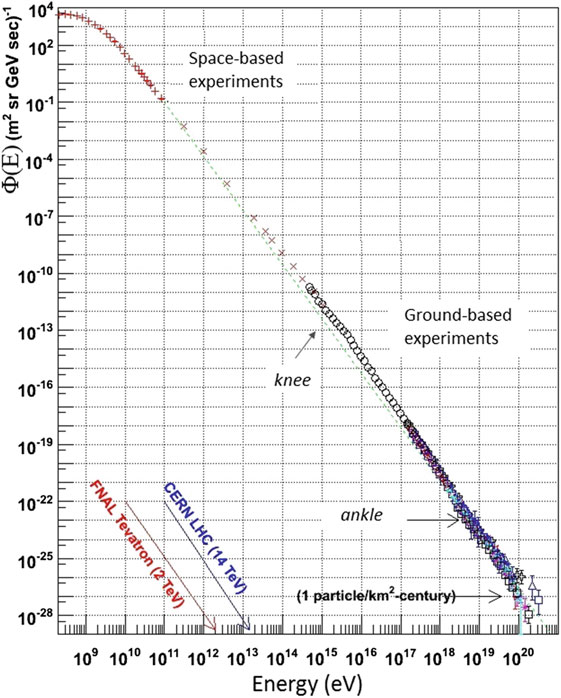
\includegraphics[width=0.7\textwidth]{Figs/differential_flux.png}
        \end{center}
       \caption[Espectro diferencial de rayos cósmicos como función de la energía]{Espectro diferencial de rayos cósmicos como función de la energía \parencite{mauro:oxigen}. Se ha elevado a la potencia 2.6 para hacer más notables los cambios en la pendiente del espectro. Se distinguen entonces la rodilla ($10^{15}eV$), tobillo ($10^{18}eV$) y corte ($10^{19}eV $). La gráfica es construida a partir de diferentes observatorios que miden directa o indirectamente en un rango de energías específico. Las grandes barras de error entre $10^{18}$ a $10^{20}$ eV se debe a que la incidencia de partículas en estos rangos de energía tiene mucha menor ocurrencia.}
       \label{fig:fig1}
    \end{figure}

%%%%%%%
La detección directa de los primarios se puede realizar en la región de bajas energías hasta $\approx 10^{14} $eV \parencite{mauro:oxigen}. Aquí detectores en satélites pueden identificar partículas individuales, separar diferentes isótopos del mismo elemento y discernir entre energía, carga y masa . Por encima de los $10^{14} $eV el flujo de partículas primarias está por debajo de decenas de partículas por metro cuadrado al año, lo que disminuye la probabilidad de detectarlas directamente.\\

Sin embargo, los primarios al llegar a la atmósfera, interactúan con los núcleos del aire, y producen otras partículas con menos energía, llamadas secundarias. Este fenómeno se produce en cadena desde el punto más alto de la atmósfera hasta que, finalmente, llegan a la superficie de la Tierra partículas menos energéticas como electrones, fotones y muones. Así, la detección directa puede ser reemplazada por instrumentos a nivel del suelo que registran el rastro que deja las cascadas \parencite{AsoreyLAGO}.\\ %Los instrumentos son diseñados en base al conocimiento y análisis de los procesos físicos involucrados en la interacciones de las partículas con la atmósfera.

A este fenómeno de producción en cadena se le denomina cascada aérea extensa o EAS por sus siglas en inglés. El comportamiento de una EAS, depende de la energía, el ángulo cenital de incidencia y el tipo de primario, además de la cantidad de atmósfera atravesada, también llamada profundidad atmosférica $X$. \\

La profundidad atmosférica $X$, es un parámetro que permite estimar la cantidad de materia con la que ha interactuado el primario al penetrar en la atmósfera. La expresión:
%Se estima teniendo en cuenta desde un punto lejano hasta la posición $h$ vertical, en presencia de una determinada densidad atmosférica, que varía con la altura sobre el nivel del mar $\rho(h')$,
\begin{equation}
X_{v}= \int_{h}^{\infty} \rho (h') dh',
\label{eq:eq2}
\end{equation}
permite cuantificar la cantidad de materia que atraviesa el primario en su viaje por la atmósfera desde el punto más alto hasta el nivel del mar \parencite{mauro:oxigen}. La dependencia de la densidad con la altura, puede ser determinada analizando la atmósfera como un gas ideal. Así, la presión a una profundidad atmosférica determinada es:
\begin{equation}
P=\frac{mg}{s} = \frac{g}{s} \int^{\infty}_{h} \rho(h')S d(h') = gX_{v}.
\label{eq:eq3}
\end{equation}\\
Además, con base en la ecuación (\ref{eq:eq2}) se tiene que la densidad puede ser expresada de la forma:
\begin{equation}
\rho = -\frac{dX_{v}}{dh},
\label{eq:eq4}
\end{equation}
donde el signo negativo representa el hecho de que la densidad disminuye a medida que $h$ se incrementa. Además, la ecuación del gas ideal,
\begin{equation}
    T = \frac{MP}{k\rho},
    \label{eq:eq4c}
\end{equation}{}
relaciona la temperatura $T$ con la presión $P$ y la densidad del gas. Reemplazando las expresiones (\ref{eq:eq3}) y (\ref{eq:eq4}) se tiene:
\begin{equation}
    T(h) = -\frac{M}{k} \frac{gX_{v}}{dX_{v} /dh}.
    \label{eq:eq5}
\end{equation}{}
Donde $k$ es la constante de Boltzman y $M$ la masa molecular promedio, que se construye a partir de los porcentajes de cada uno de sus componentes y tiene un valor de $A= 14,5 g/mol$. Una primera aproximación para encontrar una expresión para la profundidad atmosférica en base al gas ideal, considerar una temperatura constante \parencite{mauro:oxigen}. Para ello tomemos en la escala en altitud, para la atmósfera, que corresponderá al incremento en la altitud para el cual la presión atmosférica decrece en un factor de $e$.  Y está representado por la expresión:
\begin{equation}
    h_{0}= \frac{kT}{Mg};
    \label{eq:eq6}
\end{equation}{}
Usando el valor de $M$ para la superficie de la Tierra, y una temperatura aproximada de $290 K$, $h_{0} = 8.4 km$. En la región donde las astropartículas interactúan, la temperatura está entre $210 K - 240 K$ y $h_{0} = 6 km - 7 km$.
Por lo anterior, podemos encontrar el valor de la profundidad atmosférica como:
\begin{equation}
    X_{v} = X_{v}^{atm} e^{-h/h_{0}};
    \label{eq:eq7}
\end{equation}
Con $X_{v}^{atm} = 1030 g/cm^{2}$.
Considerando la curvatura terrestre y un ángulo cenital $\theta$ de incidencia del primario, la relación entre $h$ y la dirección de propagación $l$ en la atmósfera es:
\begin{equation}
    h=lcos\theta + \frac{1}{2}\frac{l^2}{R_{\oplus}}sin^{2}\theta
    \label{eq:eq8}
\end{equation}{}
Así, la profundidad atmosférica para una inclinación específica es llamada \textbf{profundidad de inclinación} y corresponde a:
\begin{equation}
X(l) = \int_{l}^{\infty} \rho (h) dl,
\label{eq:eq9}
\end{equation}
donde, para ángulos cenitales, $\theta < 60 $ se puede calcular esta profundidad como \parencite{mauro:oxigen}:
\begin{equation}
X = X_{v}cos\theta \hspace{0.5cm} y  \hspace{0.5cm} \rho = \frac{X_{v}}{h_{0}}.
\label{eq:eq10}
\end{equation}\\
Otro parámetro de vital importancia es el $X_{max}$, que corresponde al valor de profundidad atmosférica, en que el número de partículas secundarias generadas alcanza su máximo. Una característica destacable, está en que es proporcional al logaritmo de la masa del primario que dio comienzo a la EAS \parencite{Xmax}. Considerando que debido las fluctuaciones en la estimación del punto de primera interacción, es difícil medir experimentalmente su masa, es de gran utilidad que a partir del $X_{max}$ ésta podría ser inferida estadísticamente \parencite{Xmax}.\\

En consecuencia, el desarrollo de una EAS también se puede caracterizar por el número de partículas generadas a una altura determinada desde un punto de referencia. En el proceso de interacción, ese punto de referencia es llamado eje de la lluvia, que corresponde a la dirección de propagación del primario inicial. Además, la sección transversal de la EAS varía en el tiempo, aumentando en los primeros metros, y disminuyendo drásticamente luego que se alcanza una energía crítica. Llegando al nivel del mar una cantidad mucho menor. Esta sección transversal es denominada frente de la lluvia. \\

La figura \ref{fig:fig2} muestra una simulación de una cascada producida por un protón de 10$^{14}$eV. La parte $(a)$ muestra el frente de la lluvia sobre el nivel del mar. La parte $(b)$ muestra el número de partículas secundarias como función de la altura en km. Se puede observar que, el mayor número de partículas se obtiene a una altura aproximada de 6 km. La parte $(c)$ muestra el número de secundarios como función de la distancia radial al eje de la lluvia.\\

\begin{figure}[htb!]
     \begin{center}
        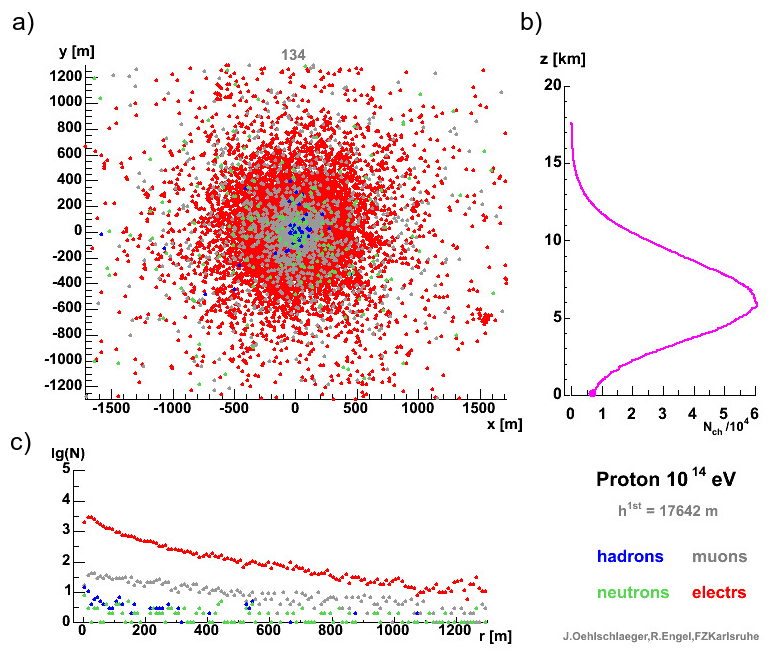
\includegraphics[width=0.7\textwidth]{Figs/frame_176_delay.png}
        \end{center}
    \caption[Simulación del desarrollo de una EAS generada por un protón de $10^{14} eV$.]{Simulación del desarrollo de una EAS generada por un protón de $10^{14} eV$ como función de la altura sobre el nivel del mar \parencite{kit}. La parte (a) muestra el frente de la lluvia, a una altura de 134m sobre el nivel del mar. La parte (b) muestra el número de partículas secundarias como función de la altura en km y la parte (c) muestra el número de secundarios como función de la distancia al eje de la lluvia.}
    \label{fig:fig2}
\end{figure}
%Figura tomada de: https://web.ikp.kit.edu/corsika
Además, teniendo en cuenta la naturaleza de las partículas secundarias, las EAS pueden clasificarse en tres constituyentes principales: la componente electromagnética, que está conformada por electrones, positrones y fotones; la componente hadrónica, constituida de piones, kaones y bariones, y la componente muónica, generada por el decaimiento de piones y kaones cargados. La figura \ref{fig:fig3} ilustra los procesos de interacción mostrados anteriormente y cómo éstos generan cada una de las componentes.
\begin{figure}[htb!]
    \begin{center}
        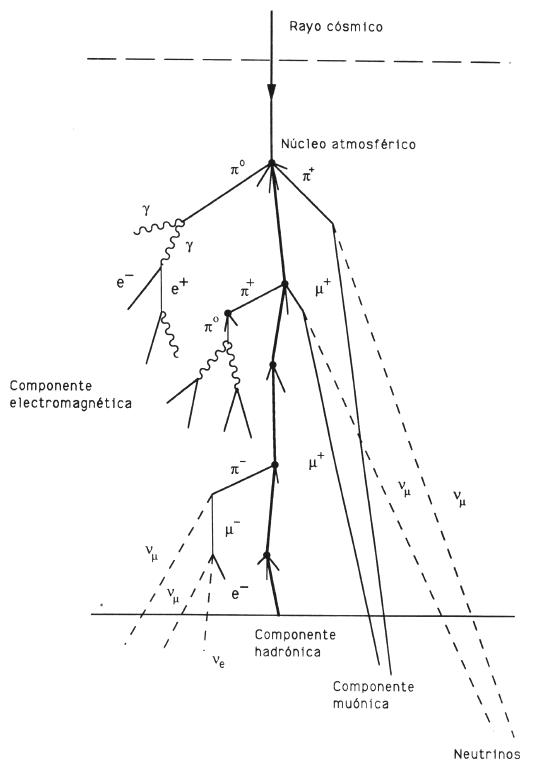
\includegraphics[width=0.6\textwidth]{Figs/componentes_cas.jpg}
    \end{center}{}
    \caption[Esquema del desarrollo de una EAS iniciada por un hadrón.]{Esquema del desarrollo más probable de una EAS iniciada por un hadrón \parencite{mauro:tesis}. En la figura se observa el decaimiento del hadrón en piones cargados y neutros, y estos a su vez, al decaer, generan fotones, electrones y muones. Se identifican tres componentes: electromagnética, muónica y hadrónica.}
    \label{fig:fig3}
\end{figure}\\
%%%%%%%%%%%%%%%%%%%%%%%%%%%
%%%%%%%%%%%%%%%%%%%%%%%%%%%%%%%%%%%%%
%      INCLUYENDO INFORMACIÓN SOBRE LA ATMÓSFERA DEL CAPÍTULO 2
%%%%%%%%%%%%%%%%%%%%%%%%%%%%%%%%%%%%%%%%%%%%%%%%%%%%%
\section{La atmósfera como medio de interacción}

Como se mencionó anteriormente, la atmósfera es un parámetro importante a la hora de estimar el flujo de secundarios, es necesario conocerla y caracterizarla adecuadamente. La atmósfera es una delgada capa gaseosa que recubre la superficie de la Tierra, principalmente compuesta por nitrógeno y oxígeno. En la tabla 1 se observan los porcentajes de abundancia de los elementos que la componen. \\

\begin{table}[htb!]
%\scriptsize
\label{tabla12}
\small
\begin{minipage}{1\textwidth}
			\caption[Composición estándar de la atmósfera.]{ \raggedright Composición estándar de la atmósfera en la superficie de la Tierra \parencite{Meteo1}.}
\end{minipage}
\begin{tabular}{cccccccl}
\hline
\multicolumn{3}{c}{\textbf{GASES PERMANENTES}} & \multicolumn{5}{c}{\textbf{GASES VARIABLES}} \\ \hline
\textbf{Gas} & \textbf{Símbolo} & \textbf{\%v/v de Aire Seco} & \textbf{Gas (y partículas)} & \textbf{Símbolo} & \textbf{\%v/v} & \multicolumn{2}{c}{\textbf{ppm}} \\ \hline
Nitrógeno & $N_{2}$ & 78.08 & Vapor de Agua & $H_{2}O$ & 0 a 4 & \multicolumn{2}{c}{} \\ \hline
Oxígeno & $O_{2}$ & 20.95 & Dióxido de Carbono & $CO_{2}$ & 0.039 & \multicolumn{2}{c}{390*} \\ \hline
Argón & $Ar$ & 0.93 & Metano & $CH_{4}$ & 0.00017 & \multicolumn{2}{c}{1.7} \\ \hline
Neon & $Ne$ & 0.0018 & Óxido nitroso & $N_{2}O$ & 0.00003 & \multicolumn{2}{c}{0.3} \\ \hline
Helio & $He$ & 0.0005 & Ozono & $O_{3}$ & 0.000004 & \multicolumn{2}{c}{0.04**} \\ \hline
Hidrógeno & $H_{2}$ & 0.00006 & Material Particulado &  & 0.000001 & \multicolumn{2}{c}{0.01-0.15} \\ \hline
Xenón & $Xe$ & 0.000009 & Clorofluorocarbonos CFCs &  & 0.00000002 & \multicolumn{2}{c}{0.0002} \\ \hline
\multicolumn{8}{l}{\multirow{2}{*}{\begin{tabular}[c]{@{}l@{}}* Para el $CO_{2}$,390 ppm  significa que de cada millón de partículas de aire, 390 son $CO_{2}$.\\\\  **Los valores estratosféricos a altitudes entre 11 y 50 km están entre los 5 y 12 ppm.\end{tabular}}} \\
\multicolumn{8}{l}{} \\ \hline
\end{tabular}
		
\end{table}

\textbf{Estructura de la atmósfera}: La atmósfera se puede clasificar por una serie de capas, estas se pueden definir de acuerdo al cambio en algunas propiedades físicas, como su temperatura, densidad, presión o sus propiedades eléctricas.\\

Para la densidad y la presión, en la figura \ref{fig:fig9} se observa una disminución a medida que se aumenta en altitud. Esto ocurre debido a la atracción gravitacional, que genera una mayor acumulación de moléculas de aire cerca de la superficie de la tierra.\\

\begin{figure}[htb!]
        \begin{center}
		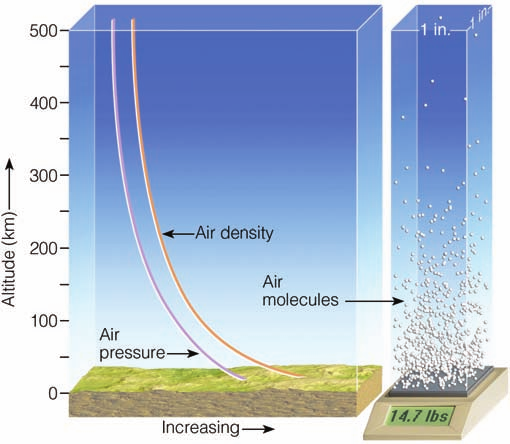
\includegraphics[width=0.6\textwidth]{Figs/PresionDensidad_vs_altitud.png}
        \end{center}
        \caption[Presión atmosférica y densidad del aire en función de la altitud.]{Comportamiento de la presión atmosférica y la densidad del aire con la altitud \parencite{Meteo1}. Se observa una relación inversa, al aumentar la altitud, la presión tiende a cero.}
        \label{fig:fig9}
\end{figure}

En cuanto a la temperatura, en la figura \ref{fig:fig10} se observa que decrece desde el suelo hasta una altura de 11 km. Esto se puede explicar porque la luz del sol calienta la superficie de la Tierra y también el aire sobre él. La tasa de cambio de la temperatura con respecto a la altura es llamado \textit{lapse rate} o gradiente adiabático. Este gradiente depende del día, la estación y la latitud.\\

La región de la atmósfera desde la superficie hasta alrededor de 11km es llamada troposfera, y contiene el clima al que estamos habituados. Allí, las moléculas de aire pueden circular a través de una profundidad de más de 10km en pocos días, y su límite se determina por la posición en el que el aire deja de enfriarse.\\

\begin{figure}[htb!]
        \begin{center}
		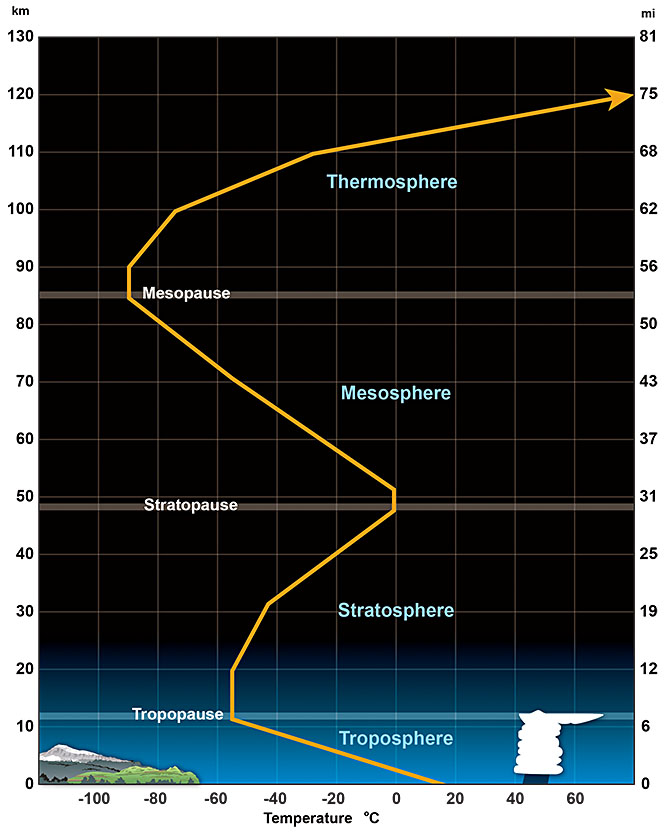
\includegraphics[width=0.6\textwidth]{Figs/atmprofile.jpg}
        \end{center}
        \caption[Temperatura promedio para las capas inferiores de la atmósfera.]{Perfil de temperatura promedio para las capas más inferiores de la atmósfera \parencite{NOAA}. Se observan las regiones de pausa, donde la temperatura permanece constante en un rango de alturas. Estas brechas marcan el final de una capa y el comienzo de otra.}
        \label{fig:fig10}
\end{figure}

Además en la figura \ref{fig:fig10}, se puede observar que entre los $\approx$10 km y los 20 km, hay una región en altitud donde la temperatura del aire se mantiene constante. Se puede inferir que el gradiente adiabático es cero, y corresponde a la tropopausa. La altura a la que se encuentra la tropopausa varía, pero es encontrada a mayor altitud en regiones ecuatoriales y decrece en dirección a los polos. Luego de la tropopausa, viene la estratosfera. Se puede observar que en esta capa la temperatura del aire comienza a incrementarse con la altura, ocurriendo una inversión.\\

La razón de esto, es que el gas ozono presente a esta altitud, tiene la función de calentar el aire, debido a que absorbe la luz solar en el ultravioleta. Así, parte de esta energía absorbida calienta la estratosfera. Si el ozono no estuviera presente, el aire probablemente podría llegar a ser más frío con la altura como en la troposfera.\\

Sobre la estratosfera ese encuentra la mesosfera. En esta capa el aire es extremadamente delgado, y la presión atmosférica es bastante baja. Sin embargo, el porcentaje de oxígeno y nitrógeno es cercano a los valores en la superficie de la Tierra. Con una temperatura promedio de -90C, es la parte mas fría de nuestra atmósfera. Finalmente se encuentra la termosfera, donde se vuelve a generar una inversión en la temperatura. Las moléculas de oxígeno absorben la luz, calentando el aire. Sin embargo, hay relativamente pocos átomos y moléculas lo que implica que la absorción de un pequeño porcentaje de energía solar, puede causar un gran incremento en la temperatura del aire. Además, es en la termosfera donde las partículas cargadas desde el Sol interactúan con las moléculas del aire produciendo las auroras. La región se extiende hasta los 500 km. \\

En consecuencia, la atmósfera no termina abruptamente en un punto, sino que va disminuyendo su densidad, tanto que la mayoría del material que la compone, se encuentra en los primeros 30 km. A pesar que aún hay moléculas que corresponden a la atmósfera cerca de los 500km, hay un límite para el cual, a cierta altitud se considera atmósfera y espacio exterior, y este límite se encuentra a $\approx$ 100km. Esta región se conoce como Línea de Karman y se puede determinar, estimando la altura a la que la densidad de la atmósfera se vuelve tan baja que la velocidad de una aeronave para conseguir una sustentación aerodinámica equivale a la velocidad orbital a esa altura.\\
%\begin{figure}[H]
 %       \begin{center}
  %      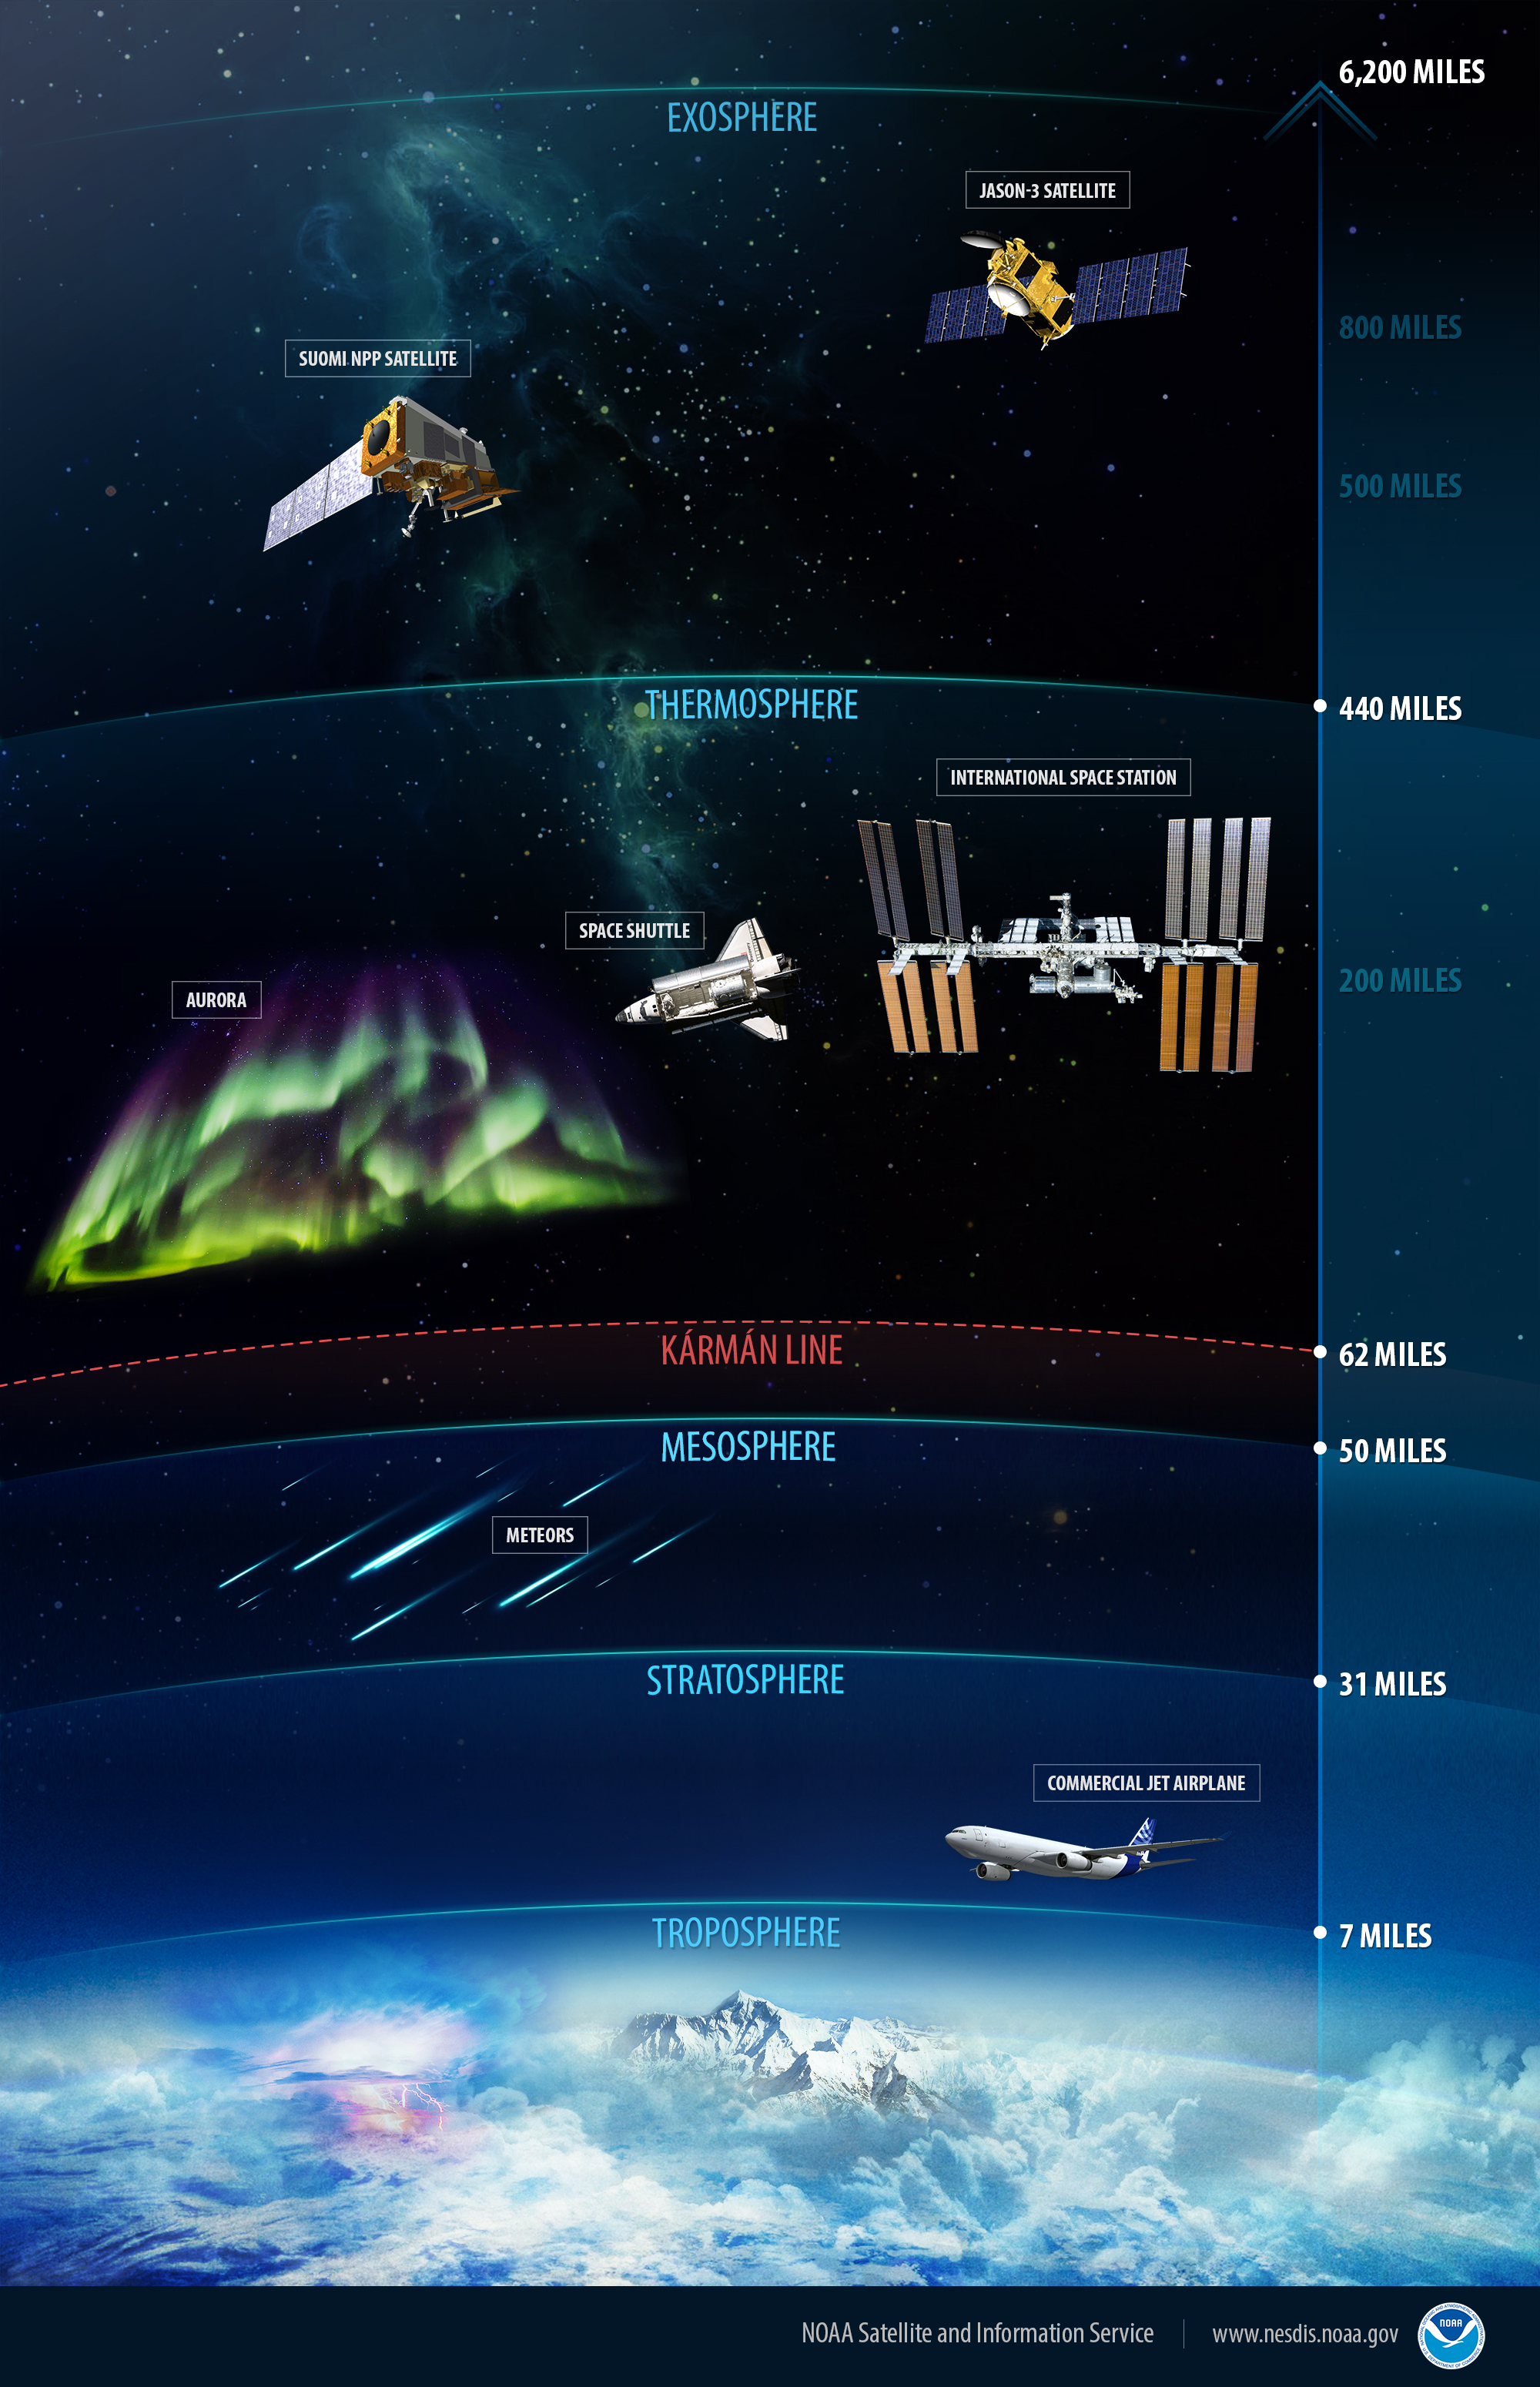
\includegraphics[width=0.7\textwidth]{Figs/Atmosphere_mid.jpg}
   %     \end{center}
    %    \caption[Representación de las capas de la atmósfera y la línea de Karman.]{Representación de las capas de la atmósfera y la línea de Karman \parencite{NOAA2}. Se pueden observar las ubicaciones de algunos  satélites, la zona donde ocurren algunos fenómenos naturales y la zona donde circulan los vuelos comerciales.}
%        \label{fig:fig11}
%\end{figure}\\
%%%%%%%%%%%%%%%%%%%%%%%%%%%%
%%%%%%%%%%%%%%%%%%%%%%%%%%%%%%%%%%%%%%%%%%%%%%
%%%%%%%%%%%%%%%%%%%%%%%%%%%%%%%%%%%%%%%%%%%%%%%%%%%%%%%%%
\section{Simulaciones de Cascadas Aéreas Extensas}
%\texbf{Punto de primera interacción}: El paso de la partícula primaria a través de la atmósfera comienza en el borde superior del modelo atmosférico. Desde este punto de partida se calcula el lugar de la primera interacción. La altura y el núcleo objetivo de esta interacción se seleccionan al azar. Opcionalmente, ambas selecciones pueden ser fijadas por valores de entrada. Las coordenadas del punto de primera interacción se establecen en (0, 0, z 0). En cada nivel de observación, las coordenadas xey se desplazan de manera que el eje de la ducha conserve las coordenadas (0, 0, z obs). Esto se hace para facilitar el análisis posterior.

Como se mencionó en secciones anteriores, el desarrollo de una EAS en la atmósfera depende de las interacciones hadrónicas y electromagnéticas de las partículas en el aire, y sus secciones eficaces de interacción. Los procesos físicos involucrados en la formación de nuevas partículas son indispensables para describir y reconstruir el fenómeno. Sin embargo, estamos ante un proceso estocástico, en el que intervienen numerosas variables y de las que es imposible determinar los valores exactos de alguno de los anteriores parámetros. De esta manera, para hacer predicciones y estimaciones relacionados con las EAS, es necesario llevar a cabo simulaciones.\\

Estas simulaciones se realizan usando el método de Monte Carlo, el cual usa números aleatorios, que modelan desarrollos físicos que pueden tener varios resultados, siguiendo una distribución de probabilidad conocida. Este tipo de análisis conduce a fluctuaciones estadísticas, de la misma forma como se observan en los datos experimentales \parencite{Alania}.\\

Un ejemplo de herramienta Monte Carlo para la simulación de EAS es CORSIKA (Cosmic Ray Simulations for Kascade). Este software es un conjunto de códigos que fueron diseñados para recrear de forma detallada cascadas aéreas extensas iniciadas por protones, fotones, núcleos o cualquier partícula que llegue a la atmósfera. CORSIKA considera las interacciones entre núcleos y las desintegraciones de estos, al interactuar con la materia. Fue desarrollado en el \textit{Karlsruhe Institute of Technology} para el experimento KASCADE, \parencite{Heck1998} y ha sido mejorado a lo largo de los años por investigadores de múltiples Institutos y Universidades del mundo. \\

CORSIKA no es el único \textit{software} que ha sido desarrollado para la simulación de EAS. Junto al desarrollo de grandes experimentos, le han acompañado la elaboración de herramientas que facilitan la interpretación de los datos. Algunos de ellos son MOCCA \parencite{Engel2018}, AIRES \parencite{Engel2018}, SENECA \parencite{Engel2018}, COSMOS \parencite{Engel2018}, GEANT4 \parencite{Engel2018} entre otros. Sin embargo, CORSIKA ha sido optimizado para la simulación de EAS y actualmente es la herramienta más utilizada y conocida para la investigación en este campo. Por esta razón, también será el software utilizado para este trabajo.\\

\textbf{Estructura general del software:} CORSIKA se compone de una gran cantidad de subrutinas que se encargan de un proceso específico dentro de la lluvia.  Además, permite al usuario seleccionar la subrutina que considere de acuerdo al fenómeno y la física involucrada que desea analizar.\\

El software está compuesto por 4 partes fundamentales. La primera se encarga del decaimiento de partículas inestables y el seguimiento de las mismas considerando las pérdidas de energía por ionización, la dispersión múltiple y el campo magnético. La segunda se encarga de las interacciones entre hadrones y la atmósfera a altas energías. La tercera parte simula las interacciones hadrónicas a bajas energías y, por último, la cuarta parte describe el transporte, la interacción de fotones y pares electrón - positrón. En las cuatro partes se han considerado todos los procesos conocidos que pudieran tener una influencia notable en las cantidades observadas de las EAS. Además contiene varios modelos para llevar a cabo las tres últimas partes que se pueden activar o desactivar opcionalmente para arrojar más detalle, o disminuyendo el tiempo de cómputo \parencite{Heck1998}. Una descripción de los códigos utilizados para la simulación de las interacciones hadrónicas y electromagnéticas se encuentran en el apéndice A.\\

Adicionalmente este código, admite la configuración de perfiles atmosféricos, predeterminados o ingresados por el usuario. Estos últimos ajustados a un momento y sitio particular. Dentro de CORSIKA, todas las partículas secundarias son rastreadas a través de sus trayectorias y sus parámetros son almacenados con una etiqueta, lo que permite un análisis detallado de las características de las lluvias simuladas.\\

Para realizar una simulación, se deben escoger una variedad de parámetros que establecen las condiciones iniciales y los límites del fenómeno que se quiere analizar. Algunos parámetros fundamentales son la naturaleza y el ángulo de incidencia del primario, el medio con el que va a interactuar, el nivel de observación, la energía o el rango de energías del primario en el espectro, la energía mínima para el seguimiento de las interacciones consecuentes y el tipo de tratamiento que se le da a la dispersión múltiple. Además, deben seleccionarse los modelos de interacciones hadrónicas y electromagnéticas.\\

CORSIKA reconoce 50 partículas elementales y núcleos atómicos hasta una masa atómica de $A = 59$. Todas las partículas que admite, pueden ser seguidas a través de la atmósfera (usando un sistema de coordenadas cartesiano). Además, son capaces de interactuar, aniquilarse, decaer y producir partículas secundarias en concordancia con el modelo estándar de física de partículas. \\

Además, opera con un generador de números aleatorios RANMAR, propuesto por Marsaglia y Zaman \parencite{RANMAR1} y modificado por F. James para el CERN \parencite{RANMAR2}. Actualmente es la herramienta estándar más usada para el análisis de fenómenos estadísticos en variados campos de aplicación incluyendo la física de partículas.\\

\textbf{Simulaci\'on de la atm\'osfera:} En CORSIKA, son de principal relevancia los perfiles de densidad que van a indicar la probabilidad de interacción a medida que evoluciona la cascada. La densidad de la atmósfera es modelada mediante 5 capas donde, para las 4 primeras capas se establece una relación exponencial:

\begin{equation}
T(h)=a_{i} + b_{i}e^{\frac{-h}{c_{i}}} \ i=1,..,4 \quad ,
\label{eq:eq25}
\end{equation}

y en la última capa, la densidad decrece linealmente con la altura de la forma:

\begin{equation}
T(h)=a_{s}-b_{s}\frac{h}{c_{s}} \ \ \mbox{ con $h_{max}$= 112.8 km} .
\label{eq:eq26}
\end{equation}


Donde $T(h)$ es la densidad de la atmósfera a una altura $h$ específica y los parámetros $a_{i}$, $b_{i}$ y $c_{i}$ se establecen de forma que la función sea continua en los límites de cada capa, y se puedan apreciar las diferencias. Se construyen entonces, varios tipos de atmósferas de tal forma que reflejen características de las diferencias estacionales \parencite{Heck1998} para una localización específica.\\

La figura \ref{fig:fig6} muestra la diferencia entre las presiones atmosféricas para distintos meses en la ciudad de Stuttgart Alemania, en comparación con la presión atmosférica estándar para Estados Unidos a diferentes altitudes. Se observa que a partir de los 30 km la diferencia entre los valores de presión disminuye a menos de 5 hPa, sin embargo hay fluctuaciones significativas a lo largo de los 30km. Estas variaciones estan relacionadas de forma directa con los perfiles de densidad.\\

Por lo anterior, CORSIKA admite tres configuraciones diferentes para el modelo atmosférico que usará en cada simulación:
\begin{itemize}
    \item MODATM, que establece atmósferas predefinidas para ubicaciones de experimentos.
    \item ATMEXT, que es una configuración para atmósferas externas dependientes de la ubicación geográfica (tropical, subtropical, ártico, etc).
    \item GDASTOOL, que genera un perfil atmosférico en base a una fecha y hora predefinidas por el usuario, usando el Sistema Global de Asimilación de Datos GDAS.
\end{itemize}{}

\begin{figure}[htb!]
\centering
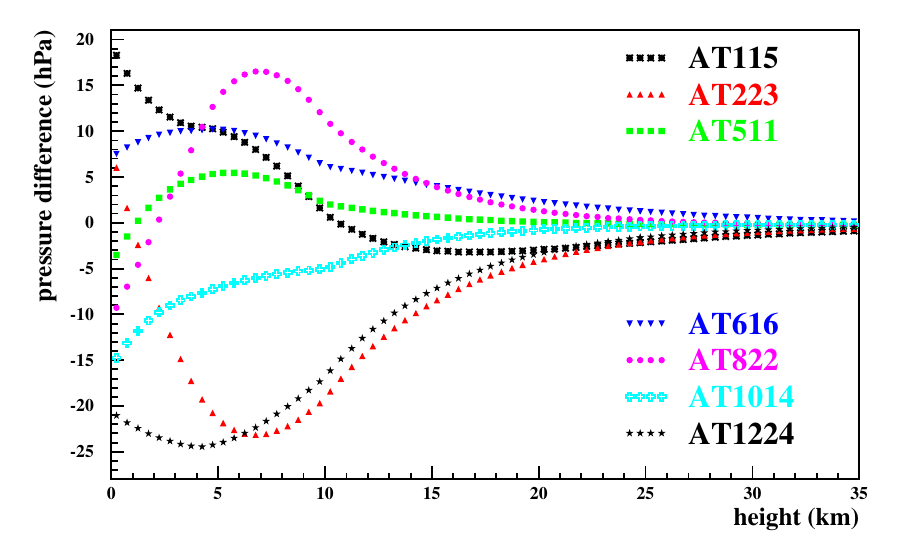
\includegraphics[width=0.7\textwidth]{Figs/ATMmodel.png}
\caption[Presión atmosférica vs la altura para Estados Unidos y Stuttgart.]{La gráfica muestra la diferencia entre las presiones atmosféricas para distintos meses en la ciudad de Stuttgart, y la presión atmosférica estándar para Estados Unidos a diferentes altitudes \parencite{Heck1998}. El modelo atmosférico AT115 corresponde al mes de enero, AT223 a febrero, AT511 a mayo, AT616 a junio, AT822 a Agosto, AT1014 corresponde a octubre y AT1224 al mes de diciembre. A cada uno de estos modelos le corresponde valores de los parámetros $a_{i}$, $b_{i}$ y $c_{i}$ característicos cuyas diferencias se ven reflejadas en las variables atmosféricas estándar, una de estas la presión, que se observa en la gráfica.}
 \label{fig:fig6}
\end{figure}
%\begin{figure}[htb!]
%\centering
%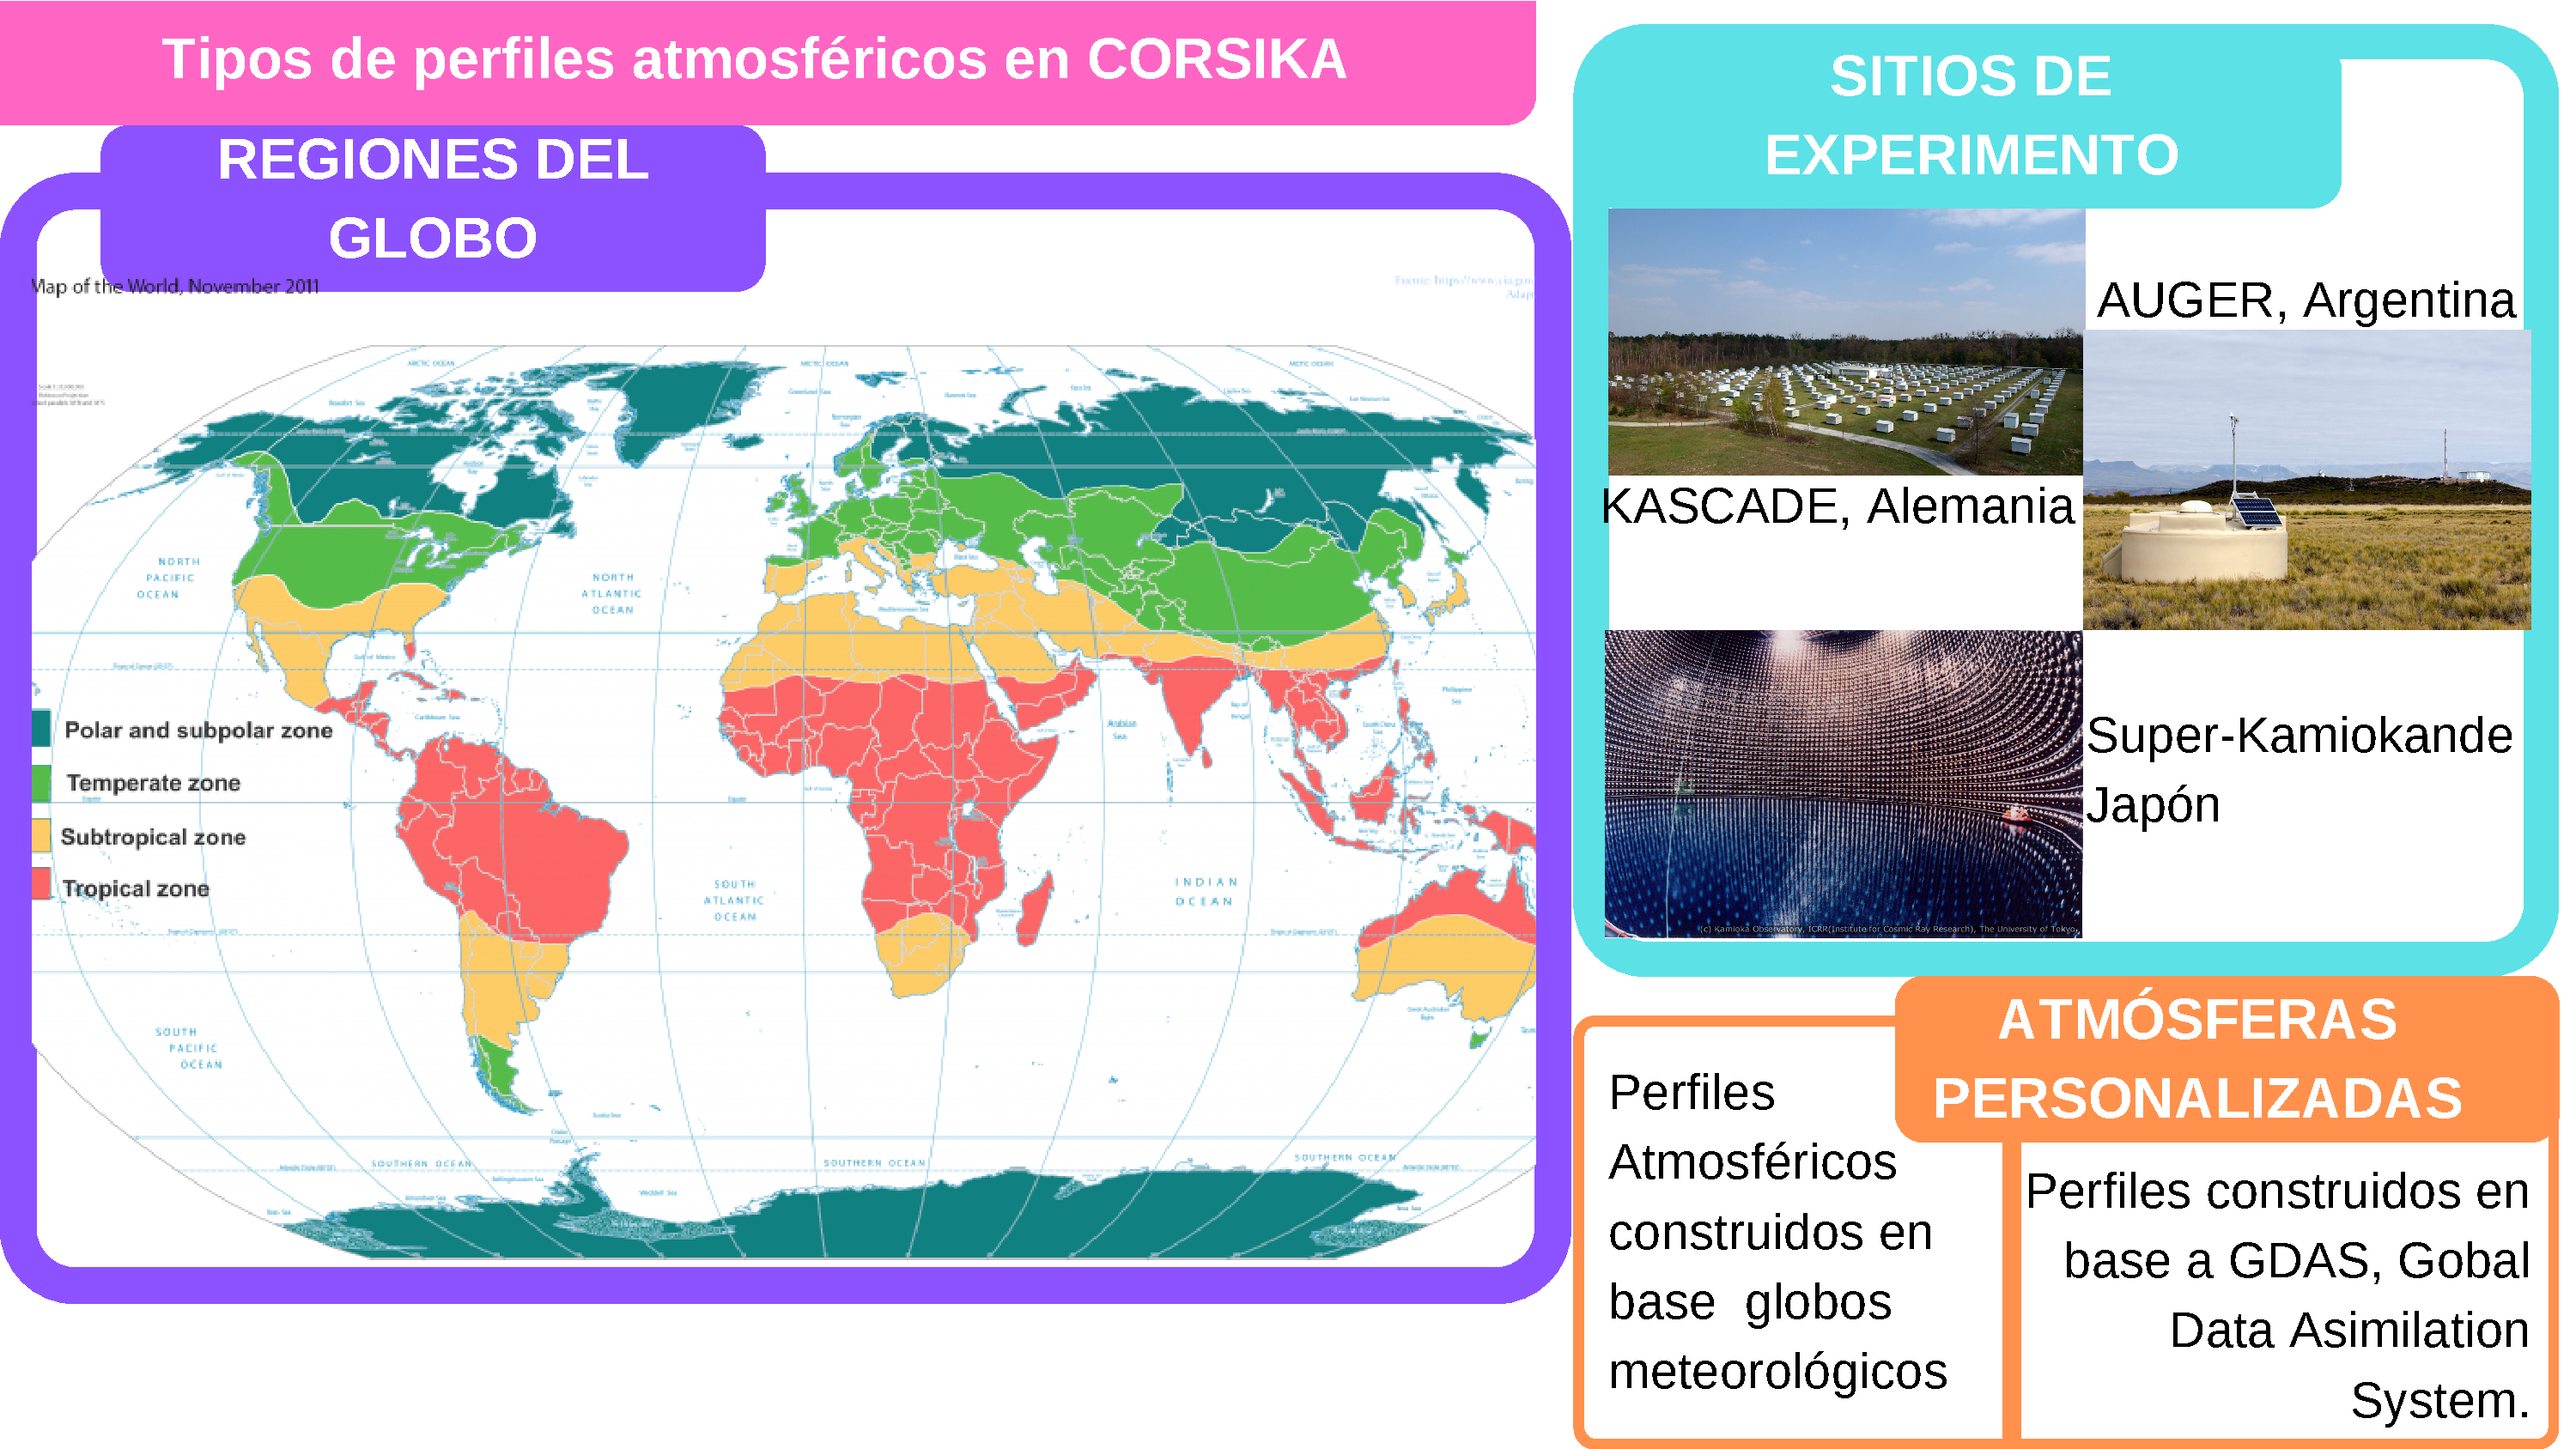
\includegraphics[width=1\textwidth]{Figs/CORSIKA_atmosfera.pdf}
%\caption[Tipos de perfiles atmosféricos que se pueden usar en CORSIKA.]{Tipos de perfiles atmosféricos que se pueden usar en CORSIKA: MODATM que establece atmósferas predefinidas para sitios estratégicos donde actualmente están ubicados observatorios de astropartículas (Cuadro superior derecho).  ATMEXT que es una configuración para atmósferas externas dependientes de la ubicación geográfica (Izquierda)  y finalmente los modelos atmosféricos construidos en base a datos o predicciones numéricas realizadas por el GDAS, que genera un perfil en base a una fecha y hora predefinidas por el usuario (Cuadro inferior izquierdo).}
% \label{fig:fig7}
%\end{figure}






